%!TEX program = xelatex

\documentclass[11pt,titlepage]{report}
%!TEX root = main.tex

\usepackage[T1]{fontenc}
\usepackage{lmodern}
\usepackage[svgnames]{xcolor}
\usepackage{fontspec} % XeLaTeX required!
\usepackage{graphicx}
\usepackage{circuitikz}
\usepackage{tikz}
\usepackage{pifont}
\usepackage[some]{background}
\usepackage{xltxtra} 
\usepackage{setspace}
\usepackage[absolute]{textpos}
\usepackage[latin1]{inputenc}
\usepackage[english]{babel}
\usepackage{graphicx}
\usepackage{wrapfig}
\usepackage{fullpage}
\usepackage[margin=1in]{geometry}
\usepackage{float}
\usepackage{url}
\usepackage{multicol}
\usepackage{hyperref}
\usepackage{titlepic}
\usepackage{standalone}
\usepackage{siunitx}
\usepackage{booktabs}
\usepackage{amsmath}
\usepackage{unicode-math}
\usepackage{verbatim}
\usepackage{enumitem}
\usepackage{listings}
\usepackage{multirow}
\usepackage{pgfplots}
\pgfplotsset{compat=1.8}
\usepackage{caption} 
\usepackage[parfill]{parskip}
\usepackage{import}
\usepackage[backend=bibtexu,texencoding=utf8,bibencoding=utf8,style=ieee,sortlocale=en_GB,language=auto]{biblatex}
\usepackage[strict,autostyle]{csquotes}
\usepackage[final]{pdfpages}
\usepackage{subcaption}
\usepackage{ifplatform}
%\captionsetup[table]{skip=10pt}


% Fix for includepdf bug in Mac OS X
\newcommand{\insertpdfpath}[1]{
	\ifwindows
	\newcommand{\insertpdf}[2]{\includepdf[pages=##1]{##2}}
	\else
	\newcommand{\insertpdf}[2]{\includepdf[pages=##1]{#1/##2}}
	\fi
}

%set fonts
\setmainfont[Ligatures=TeX]{Myriad Pro}
\setmathfont{Asana Math}
\setmonofont{Lucida Console}

\usepackage{titlesec, color}
\renewcommand{\familydefault}{\sfdefault} %set font family
\renewcommand{\arraystretch}{1.2} %set table vertical spacing
\setlength\parindent{0pt} %no paragraph indent
\hypersetup{ %setup hyperlinks
    colorlinks,
    citecolor=black,
    filecolor=black,
    linkcolor=black,
    urlcolor=black
}

%redesign chapter headings
\definecolor{gray75}{gray}{0.75}
\newcommand{\chapternumber}{\thechapter}
\newcommand{\hsp}{\hspace{20pt}}
\titleformat{\chapter}[hang]{\Huge\bfseries}{\chapternumber\hsp\textcolor{gray75}{|}\hsp}{0pt}{\Huge\bfseries}

%Redefine appendix headers
\renewcommand{\appendixname}{Appendix}
\renewcommand{\appendixtocname}{Appendices}
\renewcommand{\appendixpagename}{Appendices}

%For code listings
\definecolor{black}{rgb}{0,0,0}
\definecolor{browntags}{rgb}{0.65,0.1,0.1}
\definecolor{bluestrings}{rgb}{0,0,1}
\definecolor{graycomments}{rgb}{0.4,0.4,0.4}
\definecolor{redkeywords}{rgb}{1,0,0}
\definecolor{bluekeywords}{rgb}{0.13,0.13,0.8}
\definecolor{greencomments}{rgb}{0,0.5,0}
\definecolor{redstrings}{rgb}{0.9,0,0}
\definecolor{purpleidentifiers}{rgb}{0.01,0,0.01}


\lstdefinestyle{csharp}{
language=[Sharp]C,
showspaces=false,
showtabs=false,
breaklines=true,
showstringspaces=false,
breakatwhitespace=true,
escapeinside={(*@}{@*)},
columns=fullflexible,
commentstyle=\color{greencomments},
keywordstyle=\color{bluekeywords}\bfseries,
stringstyle=\color{redstrings},
identifierstyle=\color{purpleidentifiers},
basicstyle=\ttfamily\small}

\lstdefinestyle{c}{
language=C,
showspaces=false,
showtabs=false,
breaklines=true,
showstringspaces=false,
breakatwhitespace=true,
escapeinside={(*@}{@*)},
columns=fullflexible,
commentstyle=\color{greencomments},
keywordstyle=\color{bluekeywords}\bfseries,
stringstyle=\color{redstrings},
identifierstyle=\color{purpleidentifiers},
}

\lstdefinestyle{matlab}{
language=Matlab,
showspaces=false,
showtabs=false,
breaklines=true,
showstringspaces=false,
breakatwhitespace=true,
escapeinside={(*@}{@*)},
columns=fullflexible,
commentstyle=\color{greencomments},
keywordstyle=\color{bluekeywords}\bfseries,
stringstyle=\color{redstrings},
identifierstyle=\color{purpleidentifiers}
}

\lstdefinestyle{vhdl}{
language=VHDL,
showspaces=false,
showtabs=false,
breaklines=true,
showstringspaces=false,
breakatwhitespace=true,
escapeinside={(*@}{@*)},
columns=fullflexible,
commentstyle=\color{greencomments},
keywordstyle=\color{bluekeywords}\bfseries,
stringstyle=\color{redstrings},
identifierstyle=\color{purpleidentifiers}
}

\lstdefinestyle{xaml}{
language=XML,
showspaces=false,
showtabs=false,
breaklines=true,
showstringspaces=false,
breakatwhitespace=true,
escapeinside={(*@}{@*)},
columns=fullflexible,
commentstyle=\color{greencomments},
keywordstyle=\color{redkeywords},
stringstyle=\color{bluestrings},
tagstyle=\color{browntags},
morestring=[b]",
  morecomment=[s]{<?}{?>},
  morekeywords={xmlns,version,typex:AsyncRecords,x:Arguments,x:Boolean,x:Byte,x:Char,x:Class,x:ClassAttributes,x:ClassModifier,x:Code,x:ConnectionId,x:Decimal,x:Double,x:FactoryMethod,x:FieldModifier,x:Int16,x:Int32,x:Int64,x:Key,x:Members,x:Name,x:Object,x:Property,x:Shared,x:Single,x:String,x:Subclass,x:SynchronousMode,x:TimeSpan,x:TypeArguments,x:Uid,x:Uri,x:XData,Grid.Column,Grid.ColumnSpan,Click,ClipToBounds,Content,DropDownOpened,FontSize,Foreground,Header,Height,HorizontalAlignment,HorizontalContentAlignment,IsCancel,IsDefault,IsEnabled,IsSelected,Margin,MinHeight,MinWidth,Padding,SnapsToDevicePixels,Target,TextWrapping,Title,VerticalAlignment,VerticalContentAlignment,Width,WindowStartupLocation,Binding,Mode,OneWay,xmlns:x}
}

\lstdefinestyle{matlab}{
language=Matlab,
showspaces=false,
showtabs=false,
breaklines=true,
showstringspaces=false,
breakatwhitespace=true,
escapeinside={(*@}{@*)},
columns=fullflexible,
commentstyle=\color{greencomments},
keywordstyle=\color{bluekeywords}\bfseries,
stringstyle=\color{purpleidentifiers},
identifierstyle=\color{purpleidentifiers}
}

%defaults
\lstset{
basicstyle=\ttfamily\small,
extendedchars=false,
numbers=left,
numberstyle=\ttfamily\tiny,
stepnumber=1,
tabsize=4,
numbersep=5pt
}
\addbibresource{../../library/bibliography.bib}

\begin{document}

\section{Labday 3}
\subsection{Report 11}
For testing audio transmission, we tried to transmit some signals to see what the frequency spectrum of the received signal would be. Plots of the resulting spectra are given in Figure~\ref{fig:rep11-test-spectra}.

\begin{figure}[H]
	\centering
	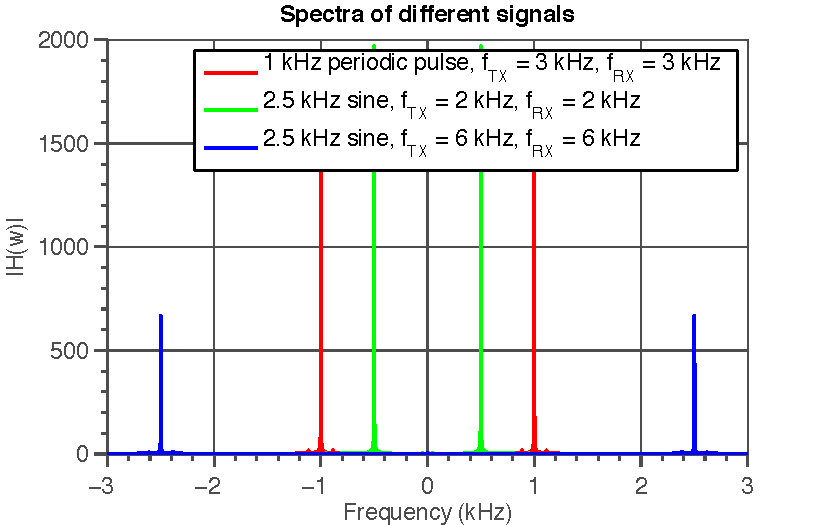
\includegraphics[width=0.6\textwidth]{../../deliverable-7-resources/figures/ass-1/report-11-12-13/ass-1-report-11-random-signals.pdf}
	\caption{Some arbitrary signal spectra, measured in the testing environment}
	\label{fig:rep11-test-spectra}
\end{figure}

We obtained mostly expected results: a sine wave sent and received with sufficient sampling rates yields delta-pulses on its positive and negative frequency and a sine wave sampled with $F_s < 2B$ results in an aliased spectrum. It is worth noting that there is not much of a difference in the spectrum of the pulsed signal, compared to that of a sine. This could be explained by speaker characteristics (a square wave requires infinite acceleration of the speaker's cone, which is not possible), as well as numerical effects due to the use of a computer system.

\begin{figure}[H]
	\centering
	\begin{subfigure}{0.49\textwidth}
		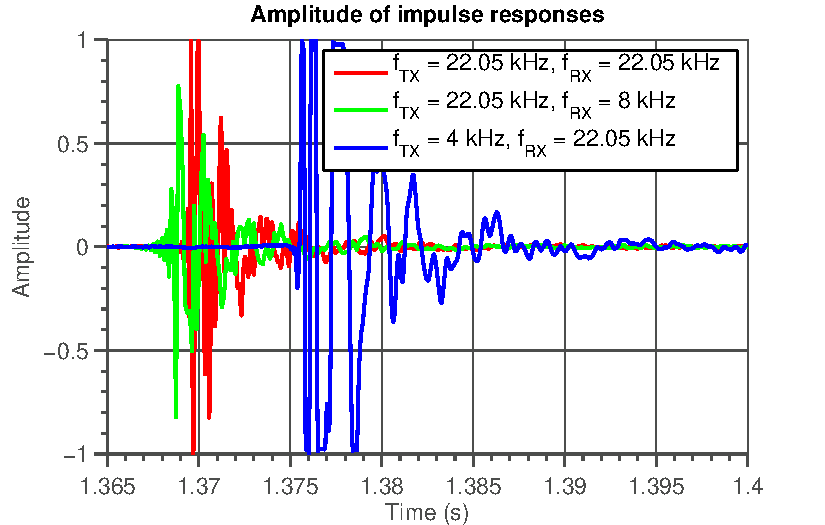
\includegraphics[width=\textwidth]{../../deliverable-7-resources/figures/ass-1/report-11-12-13/ass-1-report-11-time.pdf}
	\end{subfigure}
	\begin{subfigure}{0.49\textwidth}
		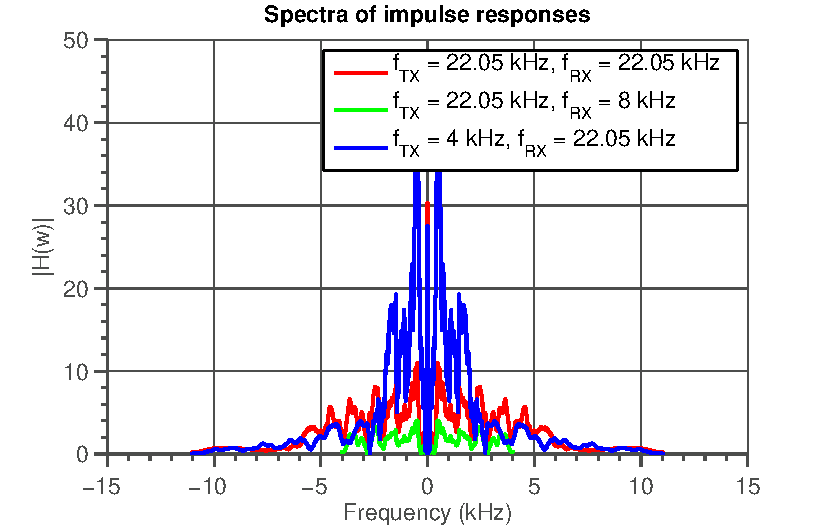
\includegraphics[width=\textwidth]{../../deliverable-7-resources/figures/ass-1/report-11-12-13/ass-1-report-11.pdf}
	\end{subfigure}
	\caption{The required impulse responses and spectra}
	\label{fig:rep11-impulse-spectra}
\end{figure}

The required impulse responses and spectra are shown in Figure~\ref{fig:rep11-impulse-spectra}. For equal $F_s$ of \SI{22,050}{\hertz}, we of course do not expect aliasing to occur. However, for $F_{s,TX} = \SI{22050}{Hz}$ and $F_{s,TX} = \SI{8000}{\hertz}$, we are clearly undersampling the received analog signal, so aliasing is to be expected. Lastly, for $F_{s,TX} = \SI{4000}{Hz}$ and $F_{s,TX} = \SI{22050}{Hz}$, we are oversampling, so aliasing is not to be expected, but the highest frequency should be $\pm \frac{F_{s,TX}}{2} = \pm \SI{2}{kHz}$, which corresponds nicely to our measured spectrum, considering the effects of noise.

%% TODO: Answer last question and check the above

\subsection{Report 12 and 13}
\label{subsec:ass1-rep-12-13}
Assuming the speed of sound to be \SI{340}{m/s}, an object that moves \SI{1}{cm} will introduce a relative delay of $0.01/340 = \SI{29.4}{\micro s}$. If we would want to detect this delay, we would need a receiver capable of a sampling rate $F_s > (29.4 \times 10^{-6})^{-1} = \SI{34}{kHz}$.

%% FIGURE subfig:rep12-time + subfig:rep12-delays IN fig:rep12-los HERE %%
\begin{figure}[H]
	\centering
	\begin{subfigure}{0.49\textwidth}
		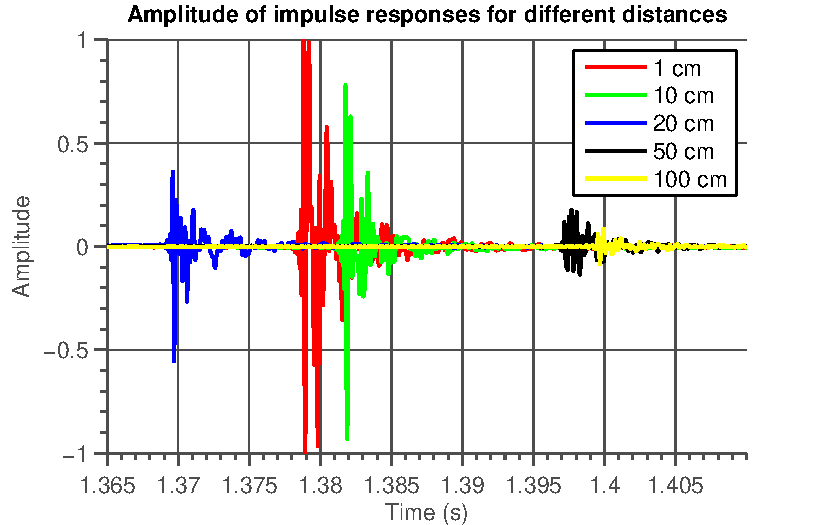
\includegraphics[width=\textwidth]{../../deliverable-7-resources/figures/ass-1/report-11-12-13/ass-1-report-13-time.pdf}
	\end{subfigure}
	\begin{subfigure}{0.49\textwidth}
		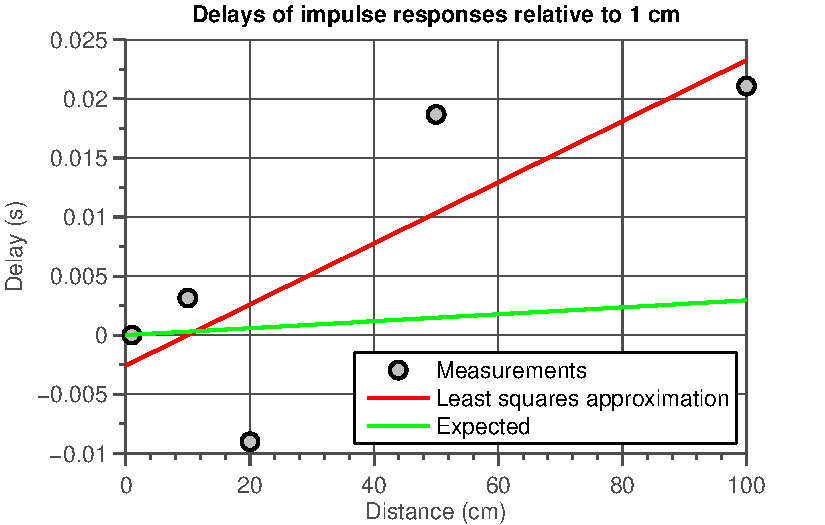
\includegraphics[width=\textwidth]{../../deliverable-7-resources/figures/ass-1/report-11-12-13/ass-1-report-13-delays.pdf}
	\end{subfigure}
	\begin{subfigure}{0.49\textwidth}
		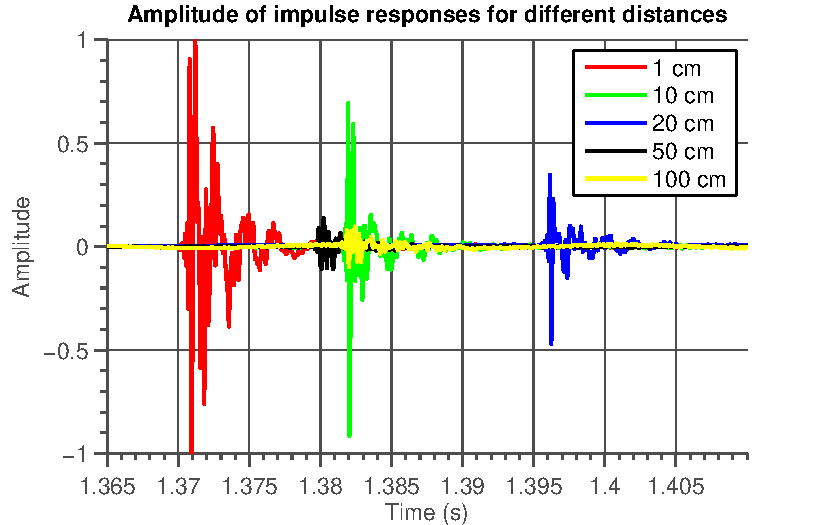
\includegraphics[width=\textwidth]{../../deliverable-7-resources/figures/ass-1/report-11-12-13/ass-1-report-13-time-set-2.pdf}
	\end{subfigure}
	\begin{subfigure}{0.49\textwidth}
		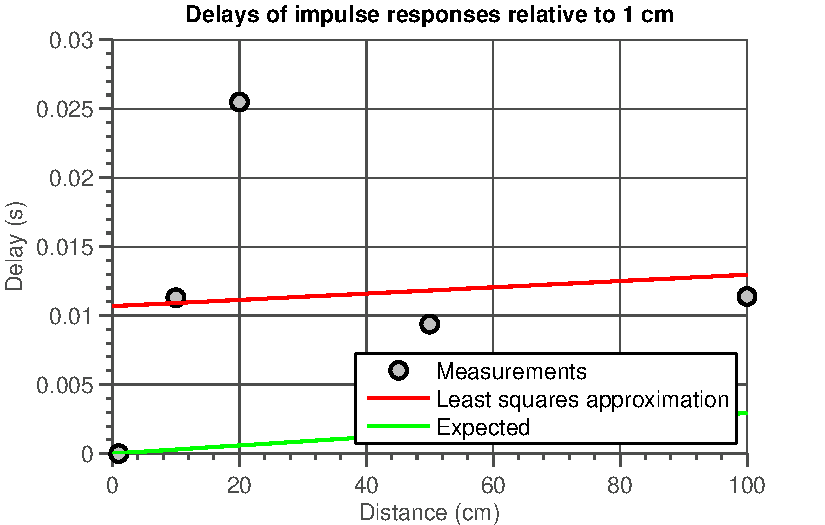
\includegraphics[width=\textwidth]{../../deliverable-7-resources/figures/ass-1/report-11-12-13/ass-1-report-13-delays-set-2.pdf}
	\end{subfigure}
	\caption{Time plots and calculated delays of the received signal, for two different measurements (top and bottom)}
	\label{fig:rep12-los}
\end{figure}

Figure~\ref{fig:rep12-los} shows time plots of the received signal after transmitting a single impulse over various distances, as well as a diagram that shows the measured delays per distance, along with an least-squares approximation and expected value line, in two measurements. Looking at the measured delays, we see that they are not all consistent with our expectations. This is most likely due to delays introduced in the processing of the received signal. When we compare the amplitudes of the various signals, we see that they indeed drop over distance, which is according to our expectations. % TODO: edit to describe two data sets

\begin{figure}[H]
	\centering
	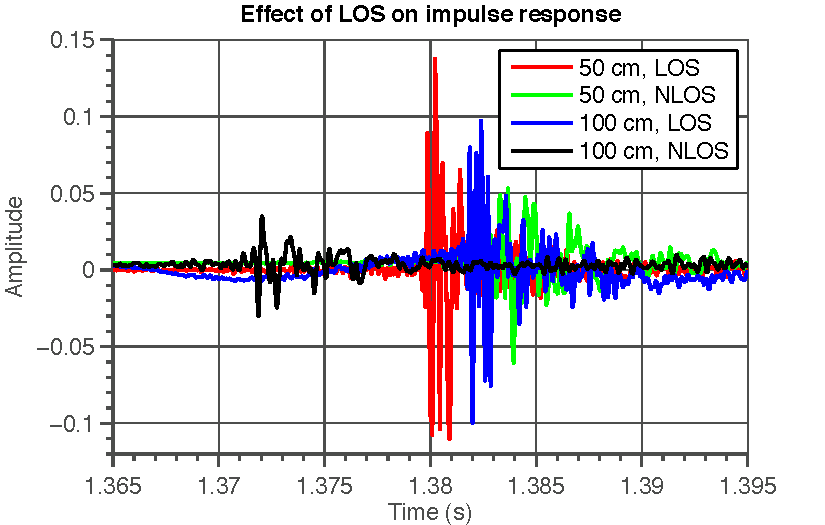
\includegraphics[width=0.8\textwidth]{../../deliverable-7-resources/figures/ass-1/report-11-12-13/ass-1-report-13-los-nlos.pdf}
	\caption{Time plots of received signals with and without line-of-sight}
	\label{fig:rep13-nlos}
\end{figure}

Repeating the previous experiment with an obstacle (a \SI{15}{"} Macbook) between the transmitter and receiver, we obtained the results as depicted in Figure~\ref{fig:rep13-nlos}. The measurements at \SI{50}{cm} show results that are to be expected, the NLOS signal was received later and with a lesser amplitude than the LOS signal. For \SI{100}{cm}, our results were less than ideal, since it looks like the NLOS signal was actually received after less time than the LOS signal, which is not conform our expectations. Once again this is probably because of processing delays in the receiver. The amplitude of the NLOS signal was indeed lower than that of the LOS signal, though.

%% TODO check the above

\subsection{Report 14}
To test our channel estimation algorithm, we sent the signal as generated by \texttt{refsignal.m}. We then recorded that signal for further processing. Both transmit- and receive sequence are shown in Figure~\ref{fig:rep14-tx-rx}.

\begin{figure}[H]
	\centering
	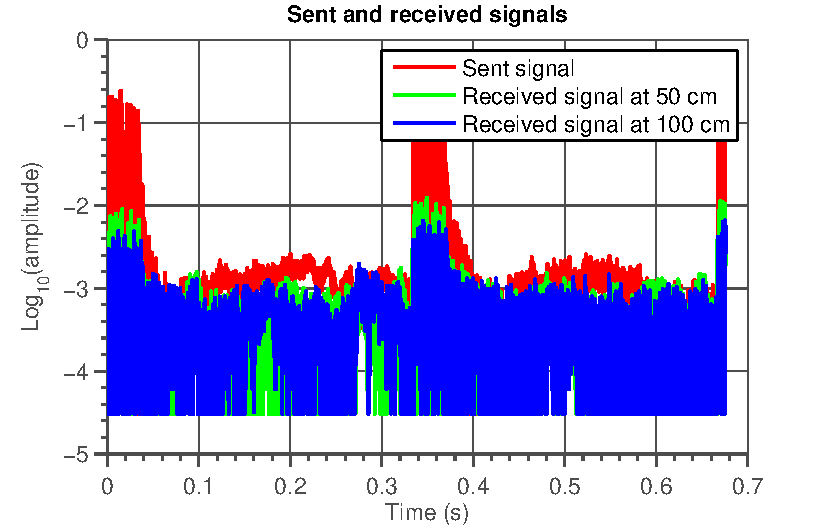
\includegraphics[width=0.8\textwidth]{../../deliverable-7-resources/figures/ass-1/report-14-15/ass-1-report-14-sent-received.pdf}
	\caption{The transmit- and receive sequence}
	\label{fig:rep14-tx-rx}
\end{figure}

These receive sequence was then processed by our channel estimation algorithm, resulting in impulse responses as shown in Figure~\ref{fig:rep14-impulse}.

\begin{figure}[H]
	\centering
	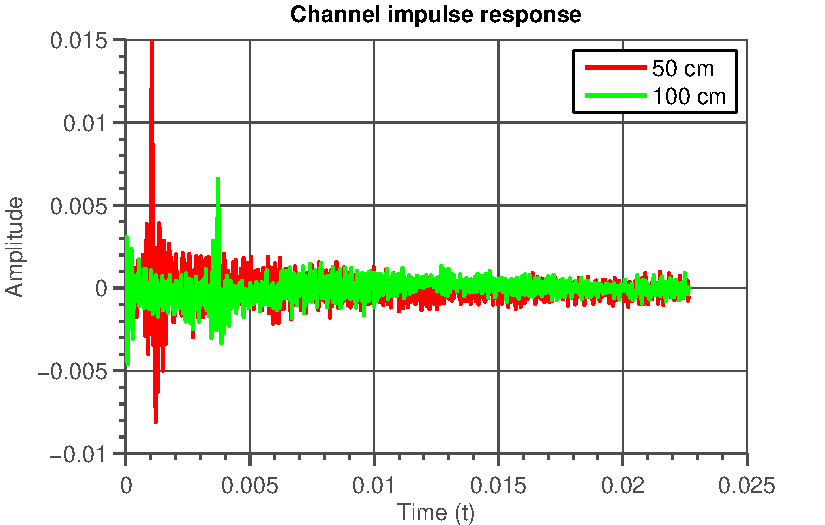
\includegraphics[width=0.8\textwidth]{../../deliverable-7-resources/figures/ass-1/report-14-15/ass-1-report-14-impulse-responses.pdf}
	\caption{The calculated impulse response for measurements, at \SI{50}{cm} and \SI{100}{cm}}
	\label{fig:rep14-impulse}
\end{figure}

To check the usability of these results, we used the obtained impulse responses to reconstruct the transmit sequence. This enabled us to make a visual comparison of the original and reconstructed sequences. Comparisons of the sequences at both measured distances are shown in Figure~\ref{fig:rep14-comparison}.

\begin{figure}[H]
	\centering
	\begin{subfigure}{0.49\textwidth}
		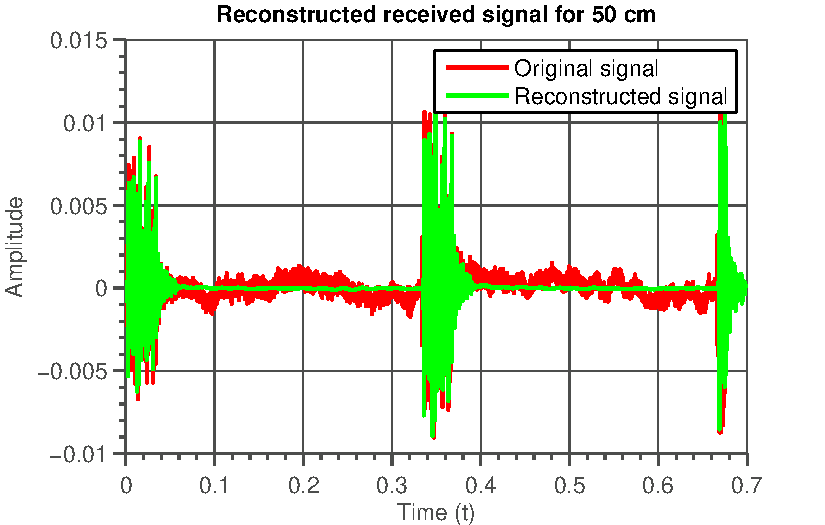
\includegraphics[width=\textwidth]{../../deliverable-7-resources/figures/ass-1/report-14-15/ass-1-report-14-50cm-reconstruction.pdf}
	\end{subfigure}
	\begin{subfigure}{0.49\textwidth}
		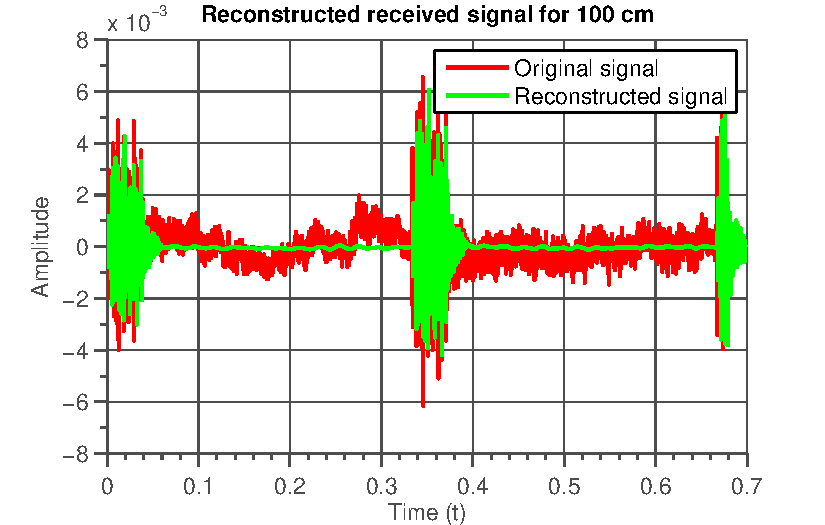
\includegraphics[width=\textwidth]{../../deliverable-7-resources/figures/ass-1/report-14-15/ass-1-report-14-100cm-reconstruction.pdf}
	\end{subfigure}
	\caption{A comparison of the original transmit sequence and the reconstructed transmit sequence, at \SI{50}{cm} and \SI{100}{cm}}
	\label{fig:rep14-comparison}
\end{figure}

We see that the reconstructed sequence mimics the original relatively well, phase and amplitude information in the peaks is mostly preserved, while at the same time noise between peaks is filtered. From these observations we may conclude that our channel estimation algorithm should be usable in TDOA localization.

\subsection{Report 15}
See section \ref{subsec:ass2-report-1} for the beacon parameters and section \ref{subsec:ass2-report5} for a motivation and background for the choice of a randomly generated $x[n]$.
\end{document}